%\section{Analysis of the function of individual hidden units}
%\label{sec:micro}
%
%\subsection{Top $K$ contexts}
%\label{sec:topk}
%
%\begin{table}[t]
%\small
%\caption{Contexts from the top 20 trigrams for example hidden units in each pathway.}
%\label{tab:contexts}
%\vspace{.2cm}
%\centering
%    \begin{tabular}{ | p{6cm} | p{6cm}|}
%    \hline
%    {\sc Visual} & {\sc Textual} \\
%    \hline
%   examples & examples  \\
%   \hline
%   \end{tabular}
%\end{table}
%
%
%The aim of this section is to develop methods that allow
%for the qualitative analysis of the kinds of linguistic features
%that individual hidden dimensions of RNNs encode. 
%We develop a simple method we dub {\it top $K$ contexts} 
%after the {\it top $K$ images} of \namecite{zhou2014object}.
%In this technique, we forward each sentence
%token by token through an RNN, and register the activation 
%of each unit in the last hidden layer of the network $\mathbf{h}_{t}$
%at each time step $t$. This results in a vector $M_i$ 
%for each hidden unit $i$, which contains  the activation of that unit 
%as a response to every token in the corpus.
%
%For each unit $i$, the entries with the highest absolute values in 
%$M_i$ represent the triggers that unit $i$ is most sensitive to. The 
%triggers could be a single token, or an n-gram including the token 
%received at the time of activation. We call such n-grams {\it top 
%contexts} of unit $i$. In this section, we analyze the top $k$ contexts
%of the hidden units to see whether they share any syntactic and/or 
%semantic patterns, indicating the function each unit is trained to perform.
%We also provide a comparison of the kinds of features the {\sc Visual} and 
%{\sc Textual} pathways of {\sc Imaginet} encode based on analysis on the 
%top $K$ contexts from the validation portion of the MS-COCO data set. 
%
%This method can be straight-forwardly applied to various 
%RNN architectures such as Elman networks or LSTMs 
%as it only requires storing the activation values for hidden units and 
%their corresponding context. For architectures with $n$ hidden layers
%one could extract multiple activation vectors $M_i^{1}, \ldots, M_i^{n}$
%for each unit, and perform analysis on each of them separately.
%A limitation of the generalizability of our analysis is that in the case of 
%bi-directional architectures the interpretation of the features
%extracted by the RNNs that process the input tokens in the reversed order
%might be hard from a linguistic point of view. 



%This involves forwarding each sentence from a corpus token-by-token through 
%an RNN, and storing the hidden activation of the network $\mathbf{h}_{t}$ 
%for each time step $t$. This results in an activation 
%matrix $M\in R^{d\times n}$, where
%$d$ is the number of hidden dimensions and $n$ is the 
%total number of time steps (or tokens) in the whole corpus. 
%Each cell $M_{it}$ in the resulting matrix represents 
%the activation value of the $i^{\text{th}}$ unit for some token at 
%time step $t$ in the corpus. 
%%Co-indexing time steps $t$ with the original sentences 
%%from the corpora allows to map the activation values of a 
%%certain neuron to a certain token in a particular context. 
%Making the assumption that high activation values indicate 
%importance, we sort the rows of the activation matrix $M$ by the 
%magnitude of the activations, leading to the top $K$ contexts for each unit.
%This method can be straight-forwardly applied to various 
%RNN architectures such as Elman networks or LSTMs 
%as it only requires storing
%the activation values for hidden units and their corresponding context.
%For architectures with $n$ hidden layers
%one could extract multiple activation matrices $M^{1}, \ldots, M^{n}$
%and perform analysis on each of them separately.
%
%In the following sections \ref{sec:topk}, \ref{sec:syntacticdim} and
%\ref{sec:carryover} we provide a qualitative exploration of the kinds of
%features the {\sc Visual} and {\sc Textual} pathways of {\sc Imaginet}
%encode based on analysis on the {\it top $K$ contexts} from the validation portion of
%the MS-COCO data set. All techniques introduced in these section can be applied
%in the same setting where {\it top $K$ contexts} can be applied.
%A limitation of the generalizability of our 
%analysis is that in the case of 
%bi-directional architectures the interpretation of the features
%extracted by the RNNs that process the input tokens in the reversed order
%might be hard from a linguistic point of view. 
%
%\subsection{Specialized hidden units}
%\label{sec:topk}
%
%Table~\ref{tab:contexts} shows the top 5 trigram contexts with the
%highest activations for five example hidden units for {\sc Visual}
%and {\sc Textual}. 
%\todo[inline]{can we explain how we chose these units, e.g. the ones with the highest maximum activation?}
%It shows the general pattern that the individual
%dimensions become highly sensitive towards contexts with syntactically
%and/or topically related patterns. 
%\todo[inline]{update the examples in Table 1 and their description below.}
%For example the top 20 trigram
%contexts for the first hidden unit of {\sc Visual} in
%Table~\ref{tab:contexts} all contain tokens topically  
%related to home electronics, such as phones, remotes and camera parts. Top-20 
%5-gram contexts for this unit include: {\it cell phone calculator and gum, 
%all hanging on wires like, such as beads and cords}. 
%
%More interestingly, the first hidden unit  for {\sc Textual} in  Table~\ref{tab:contexts}
%seems to be highly active for a combined syntactic and semantic template:
%contexts including a token corresponding to a vehicle followed by a transportation verb.
%Exploring a larger context of 5-grams reveals other interesting units 
%with high activations for such semantic/syntactic constructions in {\sc Textual}, e.g.\
%{\it a dog pokes his head, white cat sticking his head, a dog sticking its head, a dog 
%sticking his head, with a long tail perched.} 
%Further qualitative analysis on the top 50 contexts of some of the neurons {\sc Visual} shows that the model allocates certain dimensions to perform semantically informative compositions. One of the examples in Table~\ref{tab:contexts} shows that {\sc Visual} seems to learn to compose the tokens "teddy" and "bear". Another example for {\sc Visual} is a dimension, where the top context almost exclusively includes phrases with the sequence "black and white". 

%\subsection{Hidden dimensions specialized for capturing structural information}
%\label{sec:syntacticdim}
%
%Previous work \cite{} has shown during training for a specific task, that individual units (or 
%dimensions) in the hidden layers of RNNs can be specialized to capture relevant aspects of 
%information in the input. We hypothesize that some of the dimensions in the hidden layers of 
%both {\it Textual} and {\it Visual} models encode specialized structural information about the 
%utterances. 

%The aim of this section is to develop methods that allow
%for the qualitative analysis of the kinds of linguistic features
%that individual hidden dimensions of RNNs encode. 
%As discussed in the previous section, some of the analyzed units are sensitive to 
%lexical features, whereas others seem to respond to structural properties of the 
%input contexts. 

%To systematically explore the syntactic functions encoded by 
%specialized dimensions, we train two logistic regression models (one for {\sc Visual} 
%and one for {\sc Textual}) to predict the dependency label of a token at time
%step $t$. The models use two sets of predictors:
%\begin{itemize}
%  \item hidden activation vectors $\mathbf{h}_t^V$ or $\mathbf{h}_t^T$
%  \item n-gram features up to a window size of 4; for example, to predict the label 
%  for {\it dog} in the sentence {\it the nice dog}, we extract the n-gram features \{ {\it the}$_2$, {\it nice}$_1$, 
%  {\it dog}$_0$, {\it the$_2$ nice$_1$}, {\it nice$_1$ dog$_0$}, {\it the$_2$ nice$_1$ 
%  dog$_0$}\}.
%\end{itemize}
%Since the models include n-gram predictors, the logistic regression model will only
%have coefficients with high absolute values for hidden units that are predictive of 
%dependency relations over and above the n-gram features, and thus most 
%likely represent some type of functional information. Therefore, for each model 
%we pinpoint the hidden dimensions that are most predictive of each dependency label by 
%searching for the ones whose corresponding logistic regression coefficients 
%have the highest absolute value. 
%
%\begin{table}
%\small
%\caption{Examples from the top contexts for the most predictive units per dependency label in {\sc Textual} and {\sc Visual}.}
%\label{tab:syntax}
%\begin{center}
%    \begin{tabular}{|p{6cm}| p{6cm}|}
%    \hline
%   {\sc Textual} & {\sc Visual} \\
%    \hline
%    {\bf poss}:  dog sticking his, is brushing her, child brushing their, is brushing his &
%    {\bf aux}: tennis player is, racquet that is, colored ties are, but they are\\
%    \hline
%    
%    {\bf num}: several other hot, woman holding two, playing with two, group of three &
%    {\bf cc}: a waterway and, for construction or, some rocks and, with trees and\\
%    \hline
%
%    {\bf advmod}:  up a very, in a very, on a very, others watch very &
%    {\bf num}: pole in two, light with two, steeple and two, set between two\\
%    \hline
%
%   {\bf pobj}: a table covered, at a baseball, in a baseball, at a professional &
%   {\bf prep}: area surrounded by, a field with, and mountains in, the background among\\   
%       \hline
%
%   {\bf advcl}: serious while playing, standing and playing, couch while playing, as 
%he plays &
%   {\bf poss}: court holding her, player holds his, to come his, ball with her \\
%   
%   \hline
%    \end{tabular}
%\end{center}
%\end{table}
%
%
%\todo[inline]{update examples in Table 2 and their description below.}
%Table~\ref{tab:syntax} shows the top four context representations for the hidden units 
%corresponding to one of the highest coefficients for a number of the deprels for both 
%{\sc Visual} and {\sc Textual}. Some of the units in Table~\ref{tab:syntax} seem to offer 
%solely lexical cues to the deprel prediction model, while others encode more general 
%syntactic information. A number of units have high activations for target words typically 
%fulfilling the same grammatical function:
%\begin{itemize}
%    \item The example unit for the category {\sc poss} in case of {\sc Textual} has top contexts with target words {\it his, her} and {\it their}. This is also true for {\sc Visual}.
%    \item The example unit for {\sc num} for {\sc Textual} has high activations for both {\it two} and {\it three}.
%    \item The example units for {\sc cc} given for {\sc Visual} has high activations in the presence of target tokens {\it and} and {\it or}.
%    \item The contexts for the dimension of {\sc Visual} with the highest coefficient for {\sc aux} have both {\it is} and {\it are} as target tokens.
%\end{itemize}
%
%\noindent These examples, similar to the results in Section~\ref{sec:macro}, 
%highlight some of the differences between the type of linguistic 
%knowledge acquired by {\sc Textual} and {\sc Visual}. We have
%seen that {\sc Visual} learns to pay relatively more attention to contentful words
%and {\sc Textual} to words with purely grammatical function. Moreover,
%while for {\sc Textual} tokens appearing near the end of the sentence
%are more salient in general, {\sc Visual} learns to pay attention to
%sentence-initial nouns as they are likely the {\sc topic} of the sentence. 

%\subsection{Units carrying over information}
%\label{sec:carryover}
%
%Further examination of some of the highly activated units reveals dimensions
%that are predictive of deprels that require information about the
%identities or grammatical functions of previous tokens. For example,
%predictive units for {\sc pobj} in the {\sc Textual} pathway in Table~\ref{tab:syntax}
%generalize over the prepositions {\it at} and {\it in}, and contexts in the top 20 include 
%additional prepositions such as {\it around a dirt} and {\it on a grass}. But interestingly, 
%rather than being active for the prepositions themselves, all top 20 contexts belong to the 
%construction {\sc prep det pobj} where the object has to do with outdoors. 
%
%For {\sc Visual}, one of the top units for the category {\sc conj} has top contexts 
%{\it with greenery and, the table and, colored circles and, wooden furniture and, furniture 
%and a.} Given that the value of this dimension predicts the presence of a conjunct at the 
%current time step, this particular dimension seems to carry over its high activation value
%to the next time step, since all the 5 example trigrams require a
%conjunct in the next step.  This is also the case for the most predictive units of {\sc Visual} for {\sc pobj}:
%the top contexts for this unit are {\it several bunches of, with lots of, the end of, has trays 
%of} and {\it in front of}, suggesting that the information content of
%the token {\it of} must be carried over the next time step.
%
%To visually explore the phenomenon of units carrying over information through time steps, 
%we searched for interesting hidden units in {\sc Visual} using their top-20 5-gram 
%representations, and plotted their activation values through time for some example 
%captions. We only used example sentences where the activation of the hidden unit 
%was in the highest decile. Figure~\ref{fig:dimheat} shows the results.
%The first two rows are examples of \emph{lexicalized units} recognizing topically
%related words and keeping them in memory until the end of the sequence. 
%The next two rows demonstrate a hidden unit active for the multi-word expressions
%\emph{next to a} and \emph{next to an}.  The following three rows show a unit
%active for noun phrase constructions which contain a numeral followed
%by a reference to a person. 
%The last three examples show a dimension that has a modest activation for tokens of 
%category {\sc food}, but has a high activation for a following food item accompanying it in 
%the visual scene. In the very last example, the unit has a modest activation for the token 
%\emph{broccoli}, then its activation decreases for \emph{on a}. With the arrival of the token 
%\emph{plate} the activation increases again, has even higher activation for \emph{with} and 
%finally the highest for \emph{potatoes}. The top 20 5-grams for this hidden unit all contain 
%multiple food items, such as vegetables and meat with chopsticks.
%%, and compartments 
%%having fruits and vegetables such as oranges and raspberries.
%
%%Furthermore, in Section \label{sec:omitstruct} we observed 
%%that the model {\sc Visual} systematically has lower omission-scores 
%%for nouns when they have function "nn" versus when they occupy 
%%the function {\sc nsubj, pobj, dobj} or {\sc root}. 
%%The present experiment provides further evidence that {\sc Visual} 
%%recognizes "nn" as a marked grammatical function in certain contexts: some of the highest context for the top 5 coefficients for "nn" prediction involve contexts are "water fountain", "baseball player", "school bus", "wedding cake" and "traffic light". 
%
%
%
%%Another dimension in the top 5 for pobj has contexts  "attached to a, front of a, photograph of a, photo of a", where the representation of the preposition seems to be carried over two time steps.
%
%
%\begin{figure}
%\setlength{\tabcolsep}{0pt}
%\centering
%\begin{tabular}{l|r}
%
%\multirow{1}{*}{\begin{sideways}\sf tree\end{sideways}} & 
%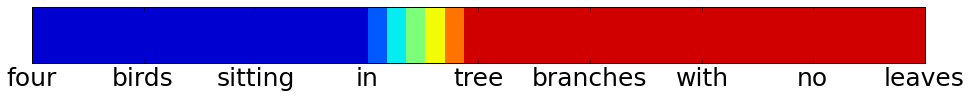
\includegraphics[scale=0.25]{dimensions/tree} \\
%\hline
%\multirow{1}{*}{\begin{sideways}\sf wii\end{sideways}} & 
% 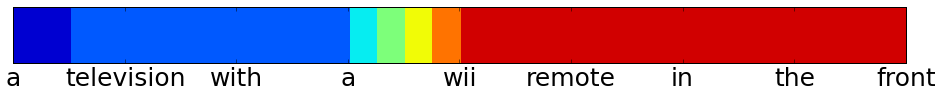
\includegraphics[scale=0.25]{dimensions/wii}  \\
%\hline
%\multirow{2}{*}{\begin{sideways}\sf next\end{sideways}} & 
%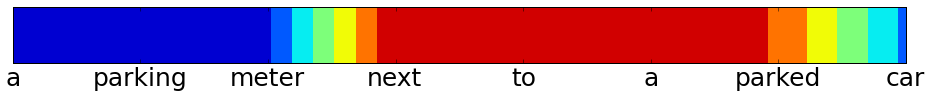
\includegraphics[scale=0.25]{dimensions/nextoacarvis} \\
%& 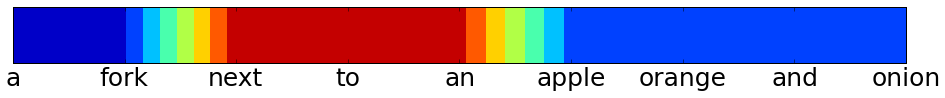
\includegraphics[scale=0.25]{dimensions/nexttoanvis}  \\
%\hline
%\hline
%\multirow{3}{*}{\begin{sideways}\sf Number\end{sideways}} & 
%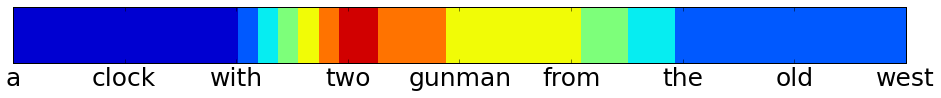
\includegraphics[scale=0.25]{dimensions/twogunmanvis}  \\
%& 
\includegraphics[scale=0.25]{dimensions/threemeneatingvis} \\
%& 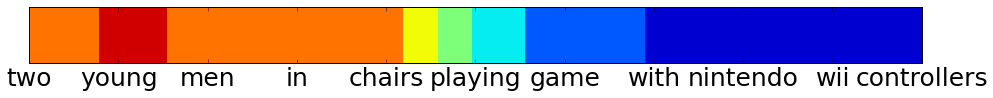
\includegraphics[scale=0.25]{dimensions/twoyoungmenvis} \\
%\hline
%\multirow{5}{*}{\begin{sideways}\sf and\end{sideways}} & 
%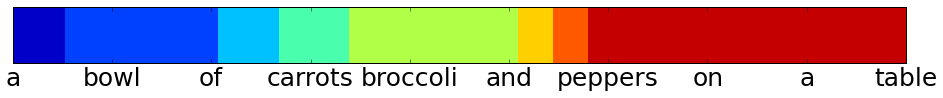
\includegraphics[scale=0.25]{dimensions/broccoliandpeppers}    \\
%& 
\includegraphics[scale=0.25]{dimensions/andgreensvis}  \\
%& 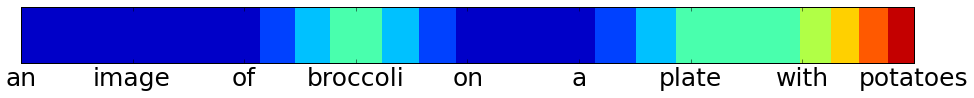
\includegraphics[scale=0.25]{dimensions/broccolipotatoes}      \\
%
%
%\end{tabular}
%
%\caption{Hidden units of {\sc Visual} active for meaningful constructions.
%The red end of the spectrum corresponds to higher activation values of the hidden unit.}
%\label{fig:dimheat}
%\end{figure}
%
\subsection{Lexical versus abstract contexts}
\label{sec:contexts}

We would like to further analyze the kinds of linguistic features that the
hidden dimensions of RNNs encode. Previous work such as 
\namecite{li2015convergent} has shown that in response 
to the task the networks are trained for, individual dimensions in the hidden layers of 
RNNs can become {\it specialised} in responding to certain types of triggers, including 
the tokens or token types at each time step, as well as the preceding context of
each token in the input sentence.
%that individual hidden dimensions of RNNs encode. 
%As discussed in the previous section, some of the analyzed units are sensitive to 
%lexical features, whereas others seem to respond to structural properties of the 
%input contexts. 

Here we explore a further comparison between the models based on the hypothesis 
that due to their different objectives, the activations of the dimensions of the last 
hidden layer of {\sc Visual} are more characterized by semantic relationships between 
the contexts, whereas the hidden dimensions in {\sc Textual} and {\sc LM} are 
more focused on extracting syntactic patterns. In order to quantitatively test this 
hypothesis, we measure the strength of association between activations of hidden 
dimensions and either lexical (token n-grams) or structural (deprel n-grams) types 
of context. 

For each pathway, we define $A_i$ as a discrete random variable corresponding 
to a binned activation over time steps at hidden dimension $i$, and $C$ 
as a discrete random variable indicating the context 
(where $C$ can be of type `word trigram' or `deprel bigram', for example). 
The strength of association between $A_i$ and $C$ can be measured 
by their mutual information:
\[
\mathrm{I}(A_i;C) = \sum_{a\in{A_i}}\sum_{c\in{C}} p(a,c)\log\left(\frac{p(a,c)}{p(a)p(c)}\right) 
\]
Similarly to \namecite{li2015convergent}, the activation value distributions are discretized 
into percentile bins per dimension, such that each bin contains 5\% of the marginal 
density. For context types, we used unigrams, bigrams and trigrams of both dependency labels 
and words. We use the notation $\mathrm{MI}^\mathit{LM}_C$,  $\mathrm{MI}^T_C$ and  $\mathrm{MI}^V_C$ 
to denote the median mutual information score over all dimensions of {\sc LM}, {\sc Textual} and {\sc Visual} 
respectively, when considering context $C$. 

% We first calculate $\mathrm{MI}^{T}_{C}$ and $\mathrm{MI}^{V}_{C}$ 
% for all six context types, and observe that the median mutual information between
% activation values of the hidden units of {\sc Textual} is higher than for {\sc Visual}.
% To statistically test the observation, we used the Wilcoxon rank-sum test and performed 
% 6 pairwise comparisons between the two models. After applying Bonferroni 
% correction we found that there is a significant difference between the models in all 
% conditions ($p< 0.008$). This suggests that in general, there is a stronger 
% relationship between the activation values of the hidden units of {\sc Textual} and the 
% n-grams they co-occur with.

We then compute log ratios $\log(\mathrm{MI}^{T}_{C}/\mathrm{MI}^{V}_{C})$ and $\log(\mathrm{MI}^\mathit{LM}_{C}/\mathrm{MI}^{T}_{C})$
for all six context types $C$. In order to quantify variability we bootstrap this statistic with
5000 replicates. Figure~\ref{fig:mi-boot} shows the resulting bootstrap distributions 
for uni-, bi-, and trigram contexts, in the word and deprel conditions. The clear pattern is 
that for {\sc Textual} versus {\sc Visual}, the log ratios are much higher in the case of the dependency contexts, with no overlap between
the bootstrap distributions. Thus, in general, the size of the
relative difference between {\sc Textual} and {\sc Visual} median
mutual information score is much more pronounced for dependency context types.
This suggests that features that are encoded by the hidden units of
the models are indeed different, and that the features encoded by {\sc Textual} are more 
associated with syntactic constructions than in the case of  {\sc
  Visual}. In contrast, when comparing {\sc LM} with {\sc Textual},
the difference between context types is much less pronounced, with
distributions overlapping. Though the difference is small, it goes in
the direction of the dimensions of the {\sc Textual} model showing
higher sensitivity towards dependency contexts.

\begin{figure}
  \centering
  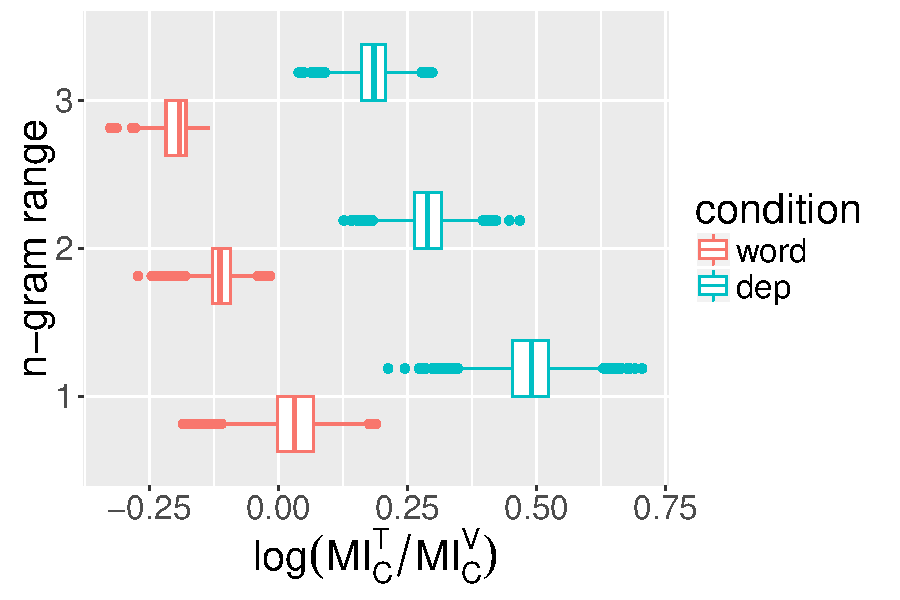
\includegraphics[scale=0.4]{bootstrappedMI.pdf}
  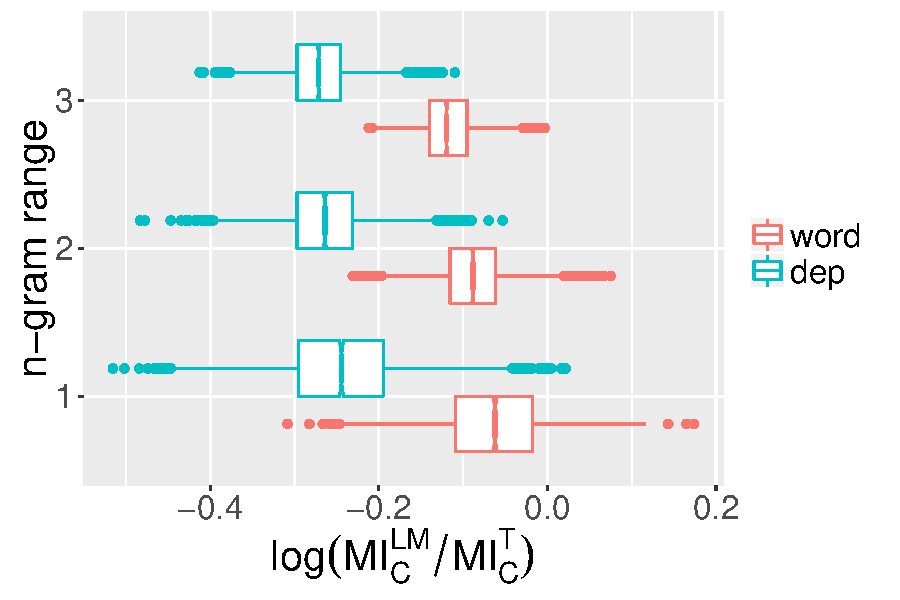
\includegraphics[scale=0.4]{bootstrappedMI2.pdf}
  \caption{Bootstrap distributions of log ratios of median mutual
    information scores for word and dependency contexts. Left: {\sc Textual}
      vs {\sc Visual}, right: {\sc LM} vs {\sc Textual}}
  \label{fig:mi-boot}
  \vspace{-.2cm}
\end{figure}


%\todo[inline]{Add and discuss sample contexts for each model here.}

The mutual information scores can be used to pinpoint specific
dimensions of the hidden activation vectors which are strongly
associated with a particular type of
context. Table~\ref{tab:mi-examples} lists for each network the
dimension with the highest mutual information score with respect to
the {\it dependency trigram} context type, together with the top
five contexts where these dimensions carry the highest value. In spite
of the quantitative difference between the networks discussed above,
the dimensions which come up top seem to be capturing something quite
similar for the three networks: (a part of) a construction with an
animate root or subject modified by a participle or a prepositional
phrase, though this is somewhat less clean-cut for the {\sc Visual}
pathway where only two out of five top context clearly conform to this
pattern.  Other interesting templates can be found by visual
inspection of the contexts where high-scoring dimensions are active:
for example dimension 324 of {\sc LM} is high for {\it word bigram} 
contexts including:
{\it people preparing, gets ready, man preparing, woman preparing,
  teenager preparing}.

\begin{table}
  \centering
\begin{tabular}{lll}
  Network            & Dimension & Examples         \\\hline
  {\sc LM}           & 511       & cookie/pobj attached/acl to/prep \\
                     &           & people/pobj sitting/acl in/prep \\
                     &           & purses/pobj sitting/pcomp on/prep\\
                     &           & and/cc talks/conj on/prep \\
                     &           & desserts/pobj sitting/acl next/advmod \\\hline
  {\sc Textual}      & 735       & male/root on/prep a/det        \\
                     &           & person/nsubj rides/root a/det   \\
                     &           & man/root carrying/acl a/det \\
                     &           & man/root on/prep a/det         \\
                     &           & person/root on/prep a/det       \\\hline
% {\sc Textual}      & dep 3 & 1008      & bears/pobj posing/acl near/prep \\
%                    &       &           & of/prep people/pobj in/prep      \\
%                    &       &           & his/poss head/dobj on/prep       \\
%                    &       &           & food/compound dish/root with/prep    \\
%                    &       &           & living/compound room/root with/prep  \\\hline
  {\sc Visual}       &  875      & man/root riding/acl a/det \\
                     &           & man/root wearing/acl a/det \\
                     &           & is/aux wearing/conj a/det \\
                     &           & a/det post/pobj next/advmod \\
                     &           & one/nummod person/nsubj is/aux \\

% {\sc LM}           & word 3 & 38        & a professional baseball \\
%                    &        &           & rustic looking living \\
%                    &        &           & a white teddy         \\
%                    &        &           & a clean living        \\
%                    &        &           & a white beige         \\\hline
%                    % & word 3 & 117       & soccer on top \\
%                    % &        &           & ball on top \\
%                    % &        &           & frisbee on top \\
%                    % &        &           & racket playing on \\
%                    % &        &           & grazing on lush \\
% {\sc Textual}      & word 3 &  764      & down a rocky \\
%                    &        &           & on a busy \\
%                    &        &           & very busy street \\
%                    &        &           & on a busy \\
%                    &        &           & is playing tennis \\\hline
% {\sc Visual}       & word 3 & 215       & electric tooth brush \\
%                    &        &           & and a girl \\
%                    &        &           & man leans down \\
%                    &        &           & little kitty laying \\
%                    &        &           & her left hand \\

\end{tabular}

\caption{Dimensions most strongly associated with the dependency trigram context type, and the top five contexts in which these dimensions have high values.} 
\label{tab:mi-examples}
\end{table}
%Figure~\ref{fig:entropybox} shows two sets of box plots representing the mutual 
%information distributions for token and deprel n-gram contexts ($n\in{1,2,3}$). 
%Results show that in fact the medians for {\sc Textual} are higher than for {\sc Visual}, 
%especially when $C$ represents deprel n-grams. This means that {\sc Textual}
%dimensions are in fact more specialized towards reacting to syntactic contexts. 




%Motivated by the intuitively interpretable context-lists describing the function of 
%hidden dimensions using the magnitude of activations values, we turn to gain more 
%insight into the difference between TEXTUAL and VISUAL. The results in Section 
%LOGISTIC suggest that the hidden representations of TEXTUAL contain more 
%information about the syntactic structure of the input sentences than VISUAL. 
%Based on this insight we conjecture that while the activity of hidden dimensions of 
%VISUAL are characterized by semantic relationships between contexts the 
%neurons of TEXTUAL are more focused on extracting syntactic patterns. To 
%validate this assumption we consider the frequency distributions of the top 10,000 
%highest activating token and dependency relation uni-, bi- and tri-gram contexts for 
%both models. Here we make two simplifying assumptions: a) as before the 
%magnitude of the activations value suggests "importance", b) we do not take into 
%consideration the rank of the contexts. We compute the entropy of these frequency 
%distributions to measure how specialized each dimensions is to specific contexts. 
%Figure \ref{fig:entropybox} compares the distribution of entropy scores of the 
%individual hidden dimensions between TEXTUAL and VISUAL. The boxplots 
%comparing the models on dependency relations - bottom row - and tokens - top row 
%- shows that in all conditions - uni-, bi-, tri-gram - the median entropy scores for the 
%hidden dimensions VISUAL are higher than for TEXTUAL. This result suggests 
%that the features extracted from the sentences by TEXTUAL resemble syntactic 
%constructions more than in case of VISUAL. To statistically test the hypothesis we 
%use the Wilcoxon rank-sum test with and perform 6 pairwise comparisons between 
%the two models on both dependency relation and token contexts. After applying 
%Bonferroni correction we find that there is a significant difference between the 
%models in all conditions except for token bi-grams - $p< 0.05/6 = 0.008$.	

%\begin{figure*}[t]

%\begin{tabular}{ccc}
%\includegraphics[scale=0.2]{unique/MItoken1} & \includegraphics[scale=0.2]
%{unique/MItoken2} & \includegraphics[scale=0.2]{unique/MItoken3} \\
%\includegraphics[scale=0.2]{unique/MIdeprel1} & \includegraphics[scale=0.2]
%{unique/MIdeprel2} & \includegraphics[scale=0.2]{unique/MIdeprel3}
%\end{tabular}

%\caption{The distribution of the Mutual Information scores for each hidden dimension of 
%{\sc Visual} and {\sc Textual}. Plots on the top row show scores for token n-grams, and on 
%the bottom row for dependency relation n-grams.}
%\label{fig:entropybox}
%\end{figure*}



